% Linear baseline — owner: Abhayanth.
% Source: notebooks/03_linear_baseline.ipynb, reports/results/linear_baseline_*.
% Include with % Linear baseline — owner: Abhayanth.
% Source: notebooks/03_linear_baseline.ipynb, reports/results/linear_baseline_*.
% Include with % Linear baseline — owner: Abhayanth.
% Source: notebooks/03_linear_baseline.ipynb, reports/results/linear_baseline_*.
% Include with % Linear baseline — owner: Abhayanth.
% Source: notebooks/03_linear_baseline.ipynb, reports/results/linear_baseline_*.
% Include with \input{sections/linear_baseline}; assumes the main file sits in
% reports/latex/ so figures resolve via ../figures/.
% Needs: graphicx, booktabs. Table: run `python reports/latex/make_tables.py` first.

\section{Linear Baseline}
\label{sec:linear_baseline}

\subsection{Method}

As a reference point for all other models, we fit linear regression with two
feature sets:
\begin{itemize}
  \item \textbf{v1 (raw, 24 features):} the 3 operating settings and 21 raw
        sensor readings of the current cycle;
  \item \textbf{v2 (engineered, 57 features):} the cycle number, the 14
        informative sensors, and a trailing 10-cycle rolling mean, standard
        deviation and slope of each (Section~\ref{sec:evaluation} explains why
        features must be causal).
\end{itemize}
Each feature is standardised (zero mean, unit variance) using statistics from
the 80 training engines only. We compare ordinary least squares (OLS) with two
regularised variants:
\begin{itemize}
  \item \textbf{Ridge}, which adds an L2 penalty $\alpha \sum_j \beta_j^2$;
  \item \textbf{Elastic Net}, which mixes L1 and L2 penalties and can set
        coefficients exactly to zero.
\end{itemize}
The same small grids were used for both feature sets to avoid overfitting the
single validation split: $\alpha \in \{0.01, 0.1, 1, 10, 100, 1000\}$ for
Ridge, and $\alpha \in \{0.001, 0.01, 0.1, 1\}$ with L1 ratio
$\in \{0.2, 0.5, 0.8\}$ for Elastic Net. Within each feature set, the setting
with the lowest validation RMSE was chosen and then scored once on the test
set.

\input{tables/linear_baseline}

\subsection{Results}

Table~\ref{tab:linear_baseline} lists the best setting of each model family.

\textbf{v2 is slightly better, and the gain comes from the cycle number.}
With v1 features, OLS, Ridge and Elastic Net all reach a validation RMSE of
42.92 cycles; OLS was kept as the simplest (test RMSE 31.17). With v2
features, Elastic Net ($\alpha = 1$, L1 ratio 0.5) reaches a validation RMSE
of 41.77 and a test RMSE of 29.04. The gain is consistent across validation,
all validation rows and test, but it is only 1--2 cycles. With about 20
independent validation engines, a gain of that size may partly be noise.

A validation-only ablation with the same model specification shows where the
gain comes from:
\begin{itemize}
  \item the cycle number plus the 14 raw sensors, with no rolling features,
        scores the same as the full v2 set (RMSE 41.74 vs.\ 41.77);
  \item removing the cycle number from v2 raises the RMSE to 43.33, slightly
        worse than v1.
\end{itemize}
For a linear model, the rolling mean, standard deviation and slope features
therefore add little once the cycle number is known. The cycle number acts as
a prior: engines that have already run longer have less life left on
average. The rolling features may still help non-linear models. The v2
Elastic Net remains the linear baseline, because it was chosen on validation
before the ablation was run.

\textbf{The linear model mostly underfits.} Training RMSE on all rows is high
for both feature sets (43.31 for v1, 39.30 for v2), so most of the error is
bias. The gap to validation widens slightly in v2 (to 47.25, against 49.72
for v1), which suggests a little more variance with 57 inputs. In v1,
regularisation therefore changes nothing. In v2 it improves on OLS by about
0.8 cycles (41.77 vs.\ 42.54). This is consistent with v2's correlated
inputs, but it is within the noise level, and the top v2 settings are
effectively tied. The best Ridge and Elastic Net strengths both lie at the
largest value tried. The grids were kept identical to v1 for comparability
and were not widened afterwards, because the test score had already been
seen.

\textbf{Uninformative and correlated inputs.} Seven raw features are constant
across the training engines (\texttt{setting\_3}, \texttt{sensor\_1},
\texttt{sensor\_5}, \texttt{sensor\_10}, \texttt{sensor\_16},
\texttt{sensor\_18} and \texttt{sensor\_19}). Seven raw feature pairs have an
absolute Pearson correlation of at least 0.8, the strongest being
\texttt{sensor\_9} and \texttt{sensor\_14} at 0.96. Individual coefficients
should therefore not be read as the effect of one sensor.

\textbf{Where the linear model fails.} For both feature sets, predictions
level off at about 150--175 cycles (Fig.~\ref{fig:linear_diagnostics}).
Engines with a true RUL between 200 and 330 cycles are predicted at roughly
130--160, and mid-range engines tend to be over-predicted.
Fig.~\ref{fig:top_sensor} suggests a likely reason. \texttt{sensor\_11}, the
raw input with the largest v1 coefficient, changes little while RUL is large;
it rises gradually from about RUL 150 and steeply near failure. A straight
line cannot represent this slow-then-accelerating pattern. This explanation
has not been tested directly. A few
predictions are negative (4 of 100 for v1, 3 of 100 for v2). They were left
unclipped, because clipping would change the model.

\textbf{Validation versus test.} Test errors are lower than validation errors
for both feature sets. A plausible but unconfirmed explanation is that the
validation cut-offs include very large RUL values that linear models miss. We
did not examine the test RUL distribution, since the protocol forbids it.

These results motivate two next steps:
\begin{itemize}
  \item non-linear models (trees) and sequence models, which can represent
        degradation that is flat and then accelerating;
  \item a capped RUL target, tested as a separate experiment.
\end{itemize}

\begin{figure}[t]
  \centering
  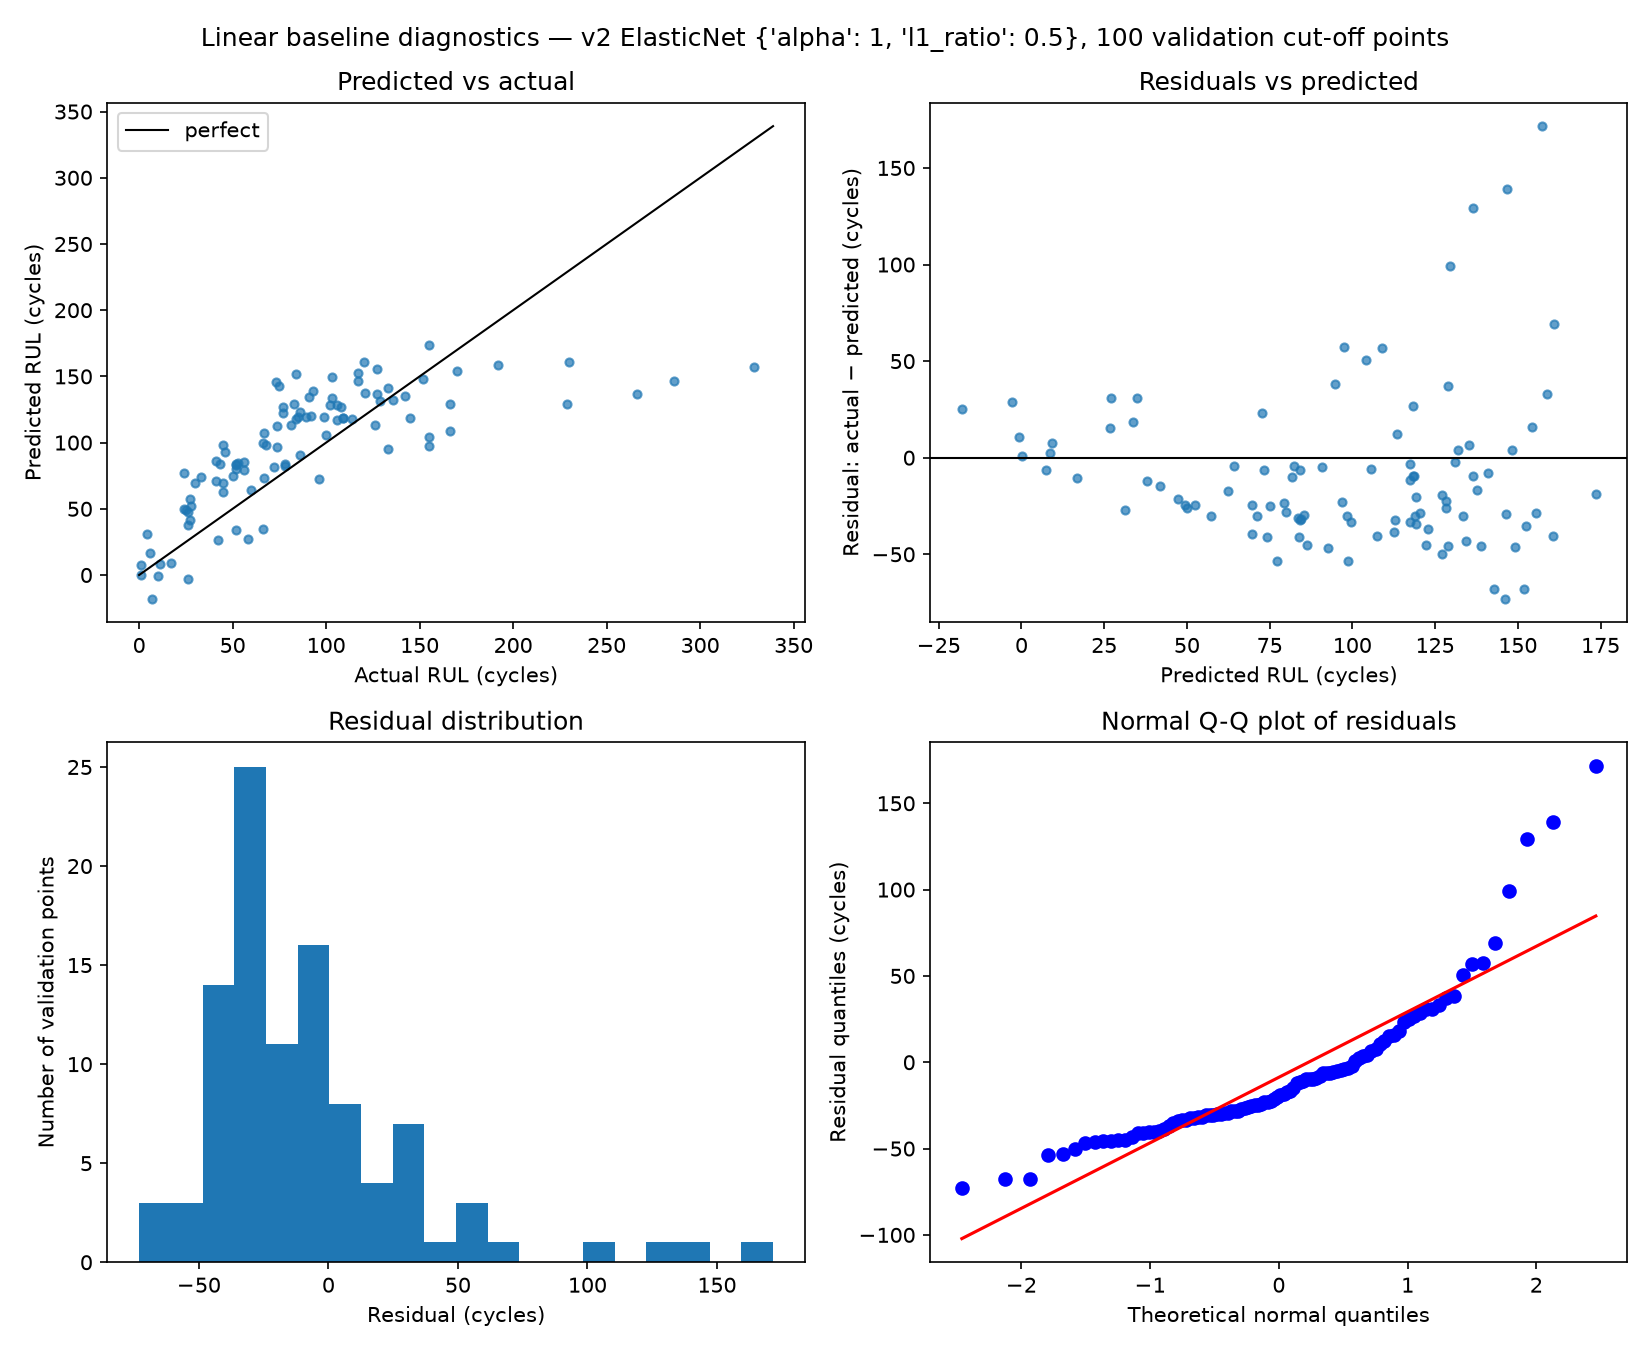
\includegraphics[width=\columnwidth]{../figures/linear_baseline_v2_validation_diagnostics.png}
  \caption{Diagnostics of the v2 linear baseline (Elastic Net) on the 100
  validation cut-off points: predicted vs.\ actual RUL, residuals vs.\
  prediction, residual histogram and normal Q-Q plot.}
  \label{fig:linear_diagnostics}
\end{figure}

\begin{figure}[t]
  \centering
  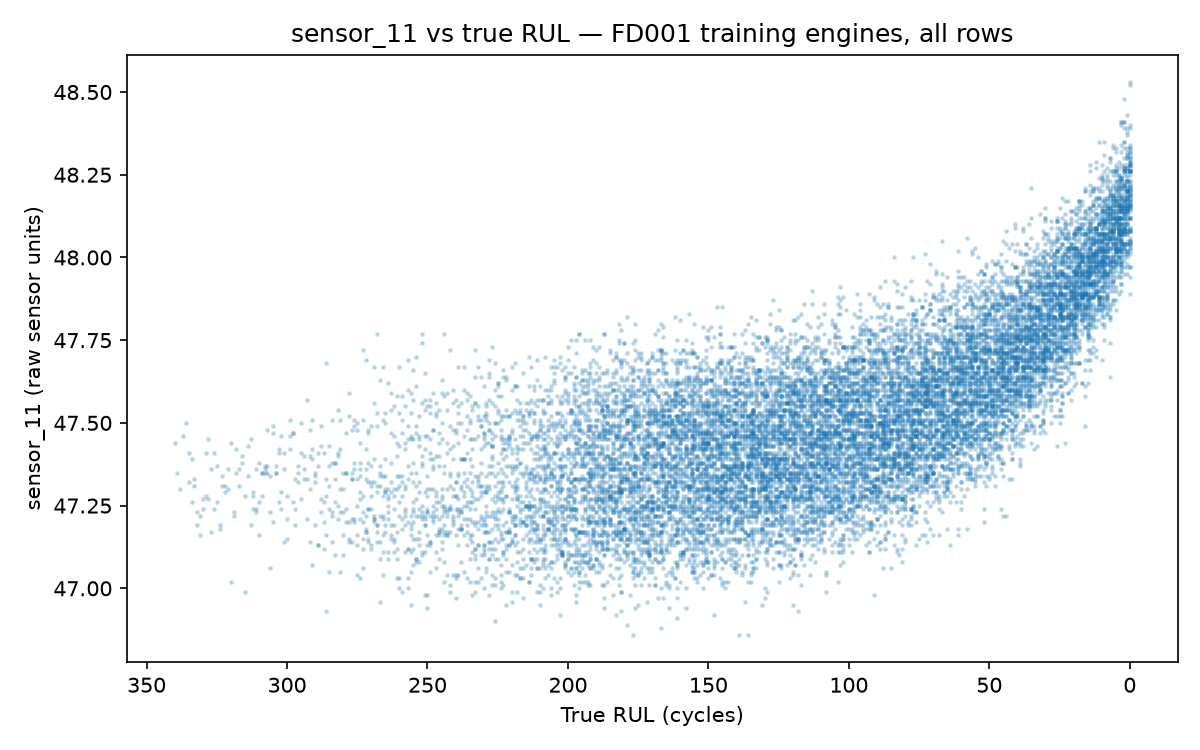
\includegraphics[width=\columnwidth]{../figures/linear_top_sensor_vs_rul.png}
  \caption{Raw \texttt{sensor\_11} against true RUL for all training rows. The
  reading changes little for large RUL and rises steeply near failure.}
  \label{fig:top_sensor}
\end{figure}
; assumes the main file sits in
% reports/latex/ so figures resolve via ../figures/.
% Needs: graphicx, booktabs. Table: run `python reports/latex/make_tables.py` first.

\section{Linear Baseline}
\label{sec:linear_baseline}

\subsection{Method}

As a reference point for all other models, we fit linear regression with two
feature sets:
\begin{itemize}
  \item \textbf{v1 (raw, 24 features):} the 3 operating settings and 21 raw
        sensor readings of the current cycle;
  \item \textbf{v2 (engineered, 57 features):} the cycle number, the 14
        informative sensors, and a trailing 10-cycle rolling mean, standard
        deviation and slope of each (Section~\ref{sec:evaluation} explains why
        features must be causal).
\end{itemize}
Each feature is standardised (zero mean, unit variance) using statistics from
the 80 training engines only. We compare ordinary least squares (OLS) with two
regularised variants:
\begin{itemize}
  \item \textbf{Ridge}, which adds an L2 penalty $\alpha \sum_j \beta_j^2$;
  \item \textbf{Elastic Net}, which mixes L1 and L2 penalties and can set
        coefficients exactly to zero.
\end{itemize}
The same small grids were used for both feature sets to avoid overfitting the
single validation split: $\alpha \in \{0.01, 0.1, 1, 10, 100, 1000\}$ for
Ridge, and $\alpha \in \{0.001, 0.01, 0.1, 1\}$ with L1 ratio
$\in \{0.2, 0.5, 0.8\}$ for Elastic Net. Within each feature set, the setting
with the lowest validation RMSE was chosen and then scored once on the test
set.

% Generated by reports/latex/make_tables.py from
% reports/results/linear_baseline_results.csv. Do not edit by hand.
\begin{table}[t]
\centering
\caption{Linear baseline on FD001 with raw (v1) and engineered (v2) features: best setting per model family. Validation: 100 cut-off points from 20 held-out engines. Test: 100 engines, scored once for the model chosen on validation within each feature set. Units: cycles.}
\label{tab:linear_baseline}
\resizebox{\columnwidth}{!}{%
\begin{tabular}{lllcccc}
\toprule
Features & Model & Hyperparameters & Val MAE & Val RMSE & Test MAE & Test RMSE \\
\midrule
v1 raw (24) & OLS & -- & 32.86 & 42.92 & 24.91 & 31.17 \\
v1 raw (24) & Ridge & $\alpha$=0.01 & 32.86 & 42.92 & -- & -- \\
v1 raw (24) & Elastic Net & $\alpha$=0.001, $\rho_{L1}$=0.8 & 32.87 & 42.92 & -- & -- \\
v2 engineered (57) & Elastic Net & $\alpha$=1, $\rho_{L1}$=0.5 & 31.66 & 41.77 & 23.61 & 29.04 \\
v2 engineered (57) & Ridge & $\alpha$=1000 & 31.93 & 41.89 & -- & -- \\
v2 engineered (57) & OLS & -- & 32.66 & 42.54 & -- & -- \\
\bottomrule
\end{tabular}}
\end{table}


\subsection{Results}

Table~\ref{tab:linear_baseline} lists the best setting of each model family.

\textbf{v2 is slightly better, and the gain comes from the cycle number.}
With v1 features, OLS, Ridge and Elastic Net all reach a validation RMSE of
42.92 cycles; OLS was kept as the simplest (test RMSE 31.17). With v2
features, Elastic Net ($\alpha = 1$, L1 ratio 0.5) reaches a validation RMSE
of 41.77 and a test RMSE of 29.04. The gain is consistent across validation,
all validation rows and test, but it is only 1--2 cycles. With about 20
independent validation engines, a gain of that size may partly be noise.

A validation-only ablation with the same model specification shows where the
gain comes from:
\begin{itemize}
  \item the cycle number plus the 14 raw sensors, with no rolling features,
        scores the same as the full v2 set (RMSE 41.74 vs.\ 41.77);
  \item removing the cycle number from v2 raises the RMSE to 43.33, slightly
        worse than v1.
\end{itemize}
For a linear model, the rolling mean, standard deviation and slope features
therefore add little once the cycle number is known. The cycle number acts as
a prior: engines that have already run longer have less life left on
average. The rolling features may still help non-linear models. The v2
Elastic Net remains the linear baseline, because it was chosen on validation
before the ablation was run.

\textbf{The linear model mostly underfits.} Training RMSE on all rows is high
for both feature sets (43.31 for v1, 39.30 for v2), so most of the error is
bias. The gap to validation widens slightly in v2 (to 47.25, against 49.72
for v1), which suggests a little more variance with 57 inputs. In v1,
regularisation therefore changes nothing. In v2 it improves on OLS by about
0.8 cycles (41.77 vs.\ 42.54). This is consistent with v2's correlated
inputs, but it is within the noise level, and the top v2 settings are
effectively tied. The best Ridge and Elastic Net strengths both lie at the
largest value tried. The grids were kept identical to v1 for comparability
and were not widened afterwards, because the test score had already been
seen.

\textbf{Uninformative and correlated inputs.} Seven raw features are constant
across the training engines (\texttt{setting\_3}, \texttt{sensor\_1},
\texttt{sensor\_5}, \texttt{sensor\_10}, \texttt{sensor\_16},
\texttt{sensor\_18} and \texttt{sensor\_19}). Seven raw feature pairs have an
absolute Pearson correlation of at least 0.8, the strongest being
\texttt{sensor\_9} and \texttt{sensor\_14} at 0.96. Individual coefficients
should therefore not be read as the effect of one sensor.

\textbf{Where the linear model fails.} For both feature sets, predictions
level off at about 150--175 cycles (Fig.~\ref{fig:linear_diagnostics}).
Engines with a true RUL between 200 and 330 cycles are predicted at roughly
130--160, and mid-range engines tend to be over-predicted.
Fig.~\ref{fig:top_sensor} suggests a likely reason. \texttt{sensor\_11}, the
raw input with the largest v1 coefficient, changes little while RUL is large;
it rises gradually from about RUL 150 and steeply near failure. A straight
line cannot represent this slow-then-accelerating pattern. This explanation
has not been tested directly. A few
predictions are negative (4 of 100 for v1, 3 of 100 for v2). They were left
unclipped, because clipping would change the model.

\textbf{Validation versus test.} Test errors are lower than validation errors
for both feature sets. A plausible but unconfirmed explanation is that the
validation cut-offs include very large RUL values that linear models miss. We
did not examine the test RUL distribution, since the protocol forbids it.

These results motivate two next steps:
\begin{itemize}
  \item non-linear models (trees) and sequence models, which can represent
        degradation that is flat and then accelerating;
  \item a capped RUL target, tested as a separate experiment.
\end{itemize}

\begin{figure}[t]
  \centering
  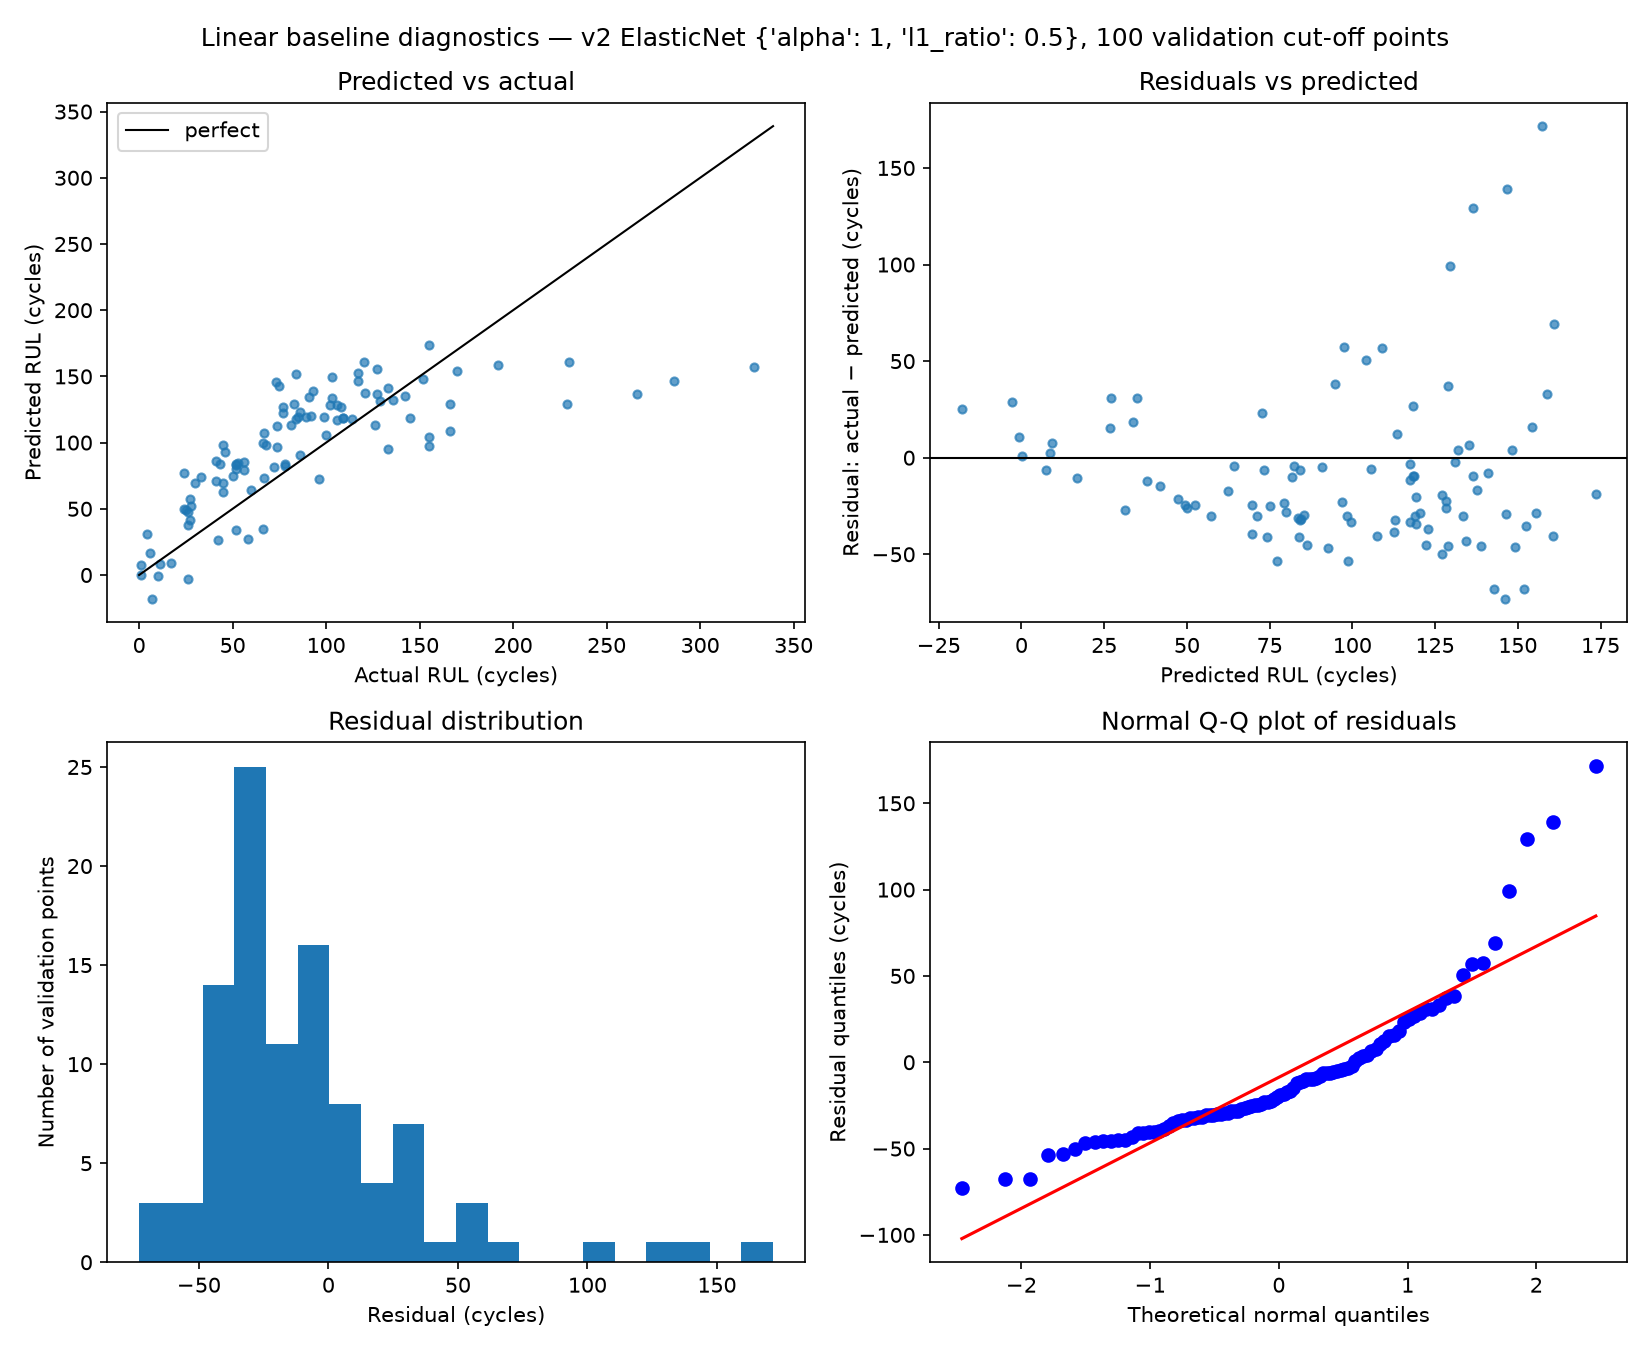
\includegraphics[width=\columnwidth]{../figures/linear_baseline_v2_validation_diagnostics.png}
  \caption{Diagnostics of the v2 linear baseline (Elastic Net) on the 100
  validation cut-off points: predicted vs.\ actual RUL, residuals vs.\
  prediction, residual histogram and normal Q-Q plot.}
  \label{fig:linear_diagnostics}
\end{figure}

\begin{figure}[t]
  \centering
  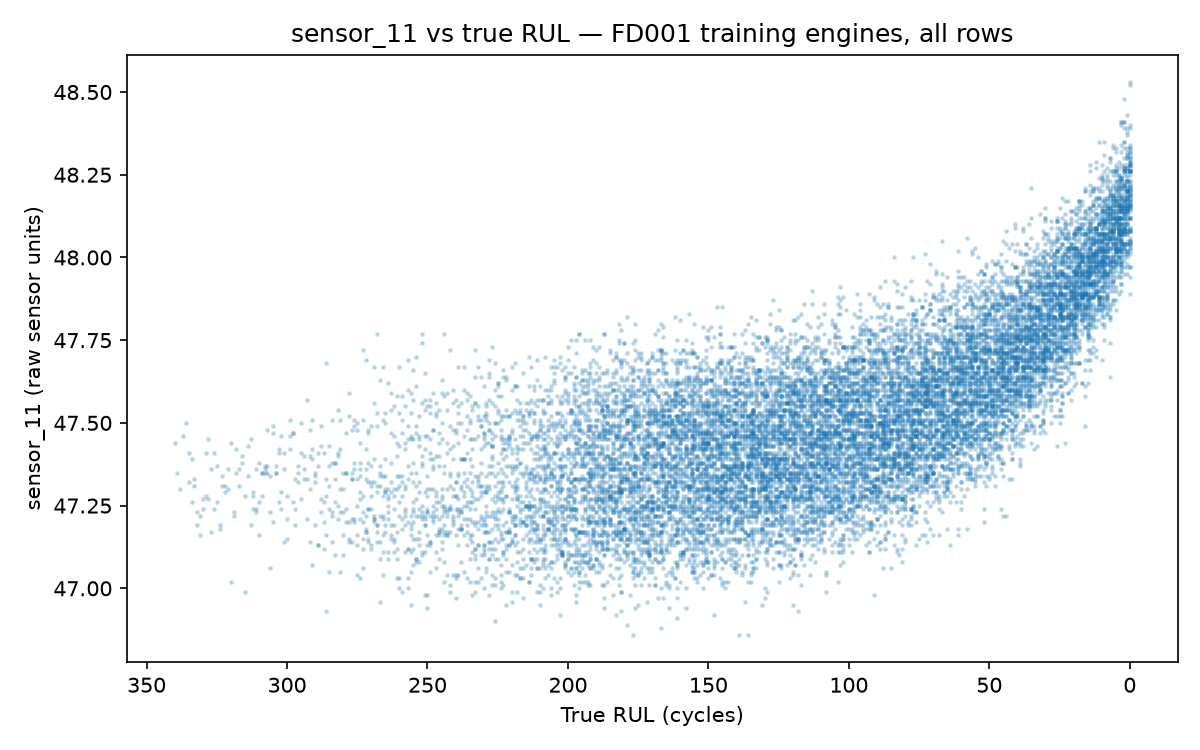
\includegraphics[width=\columnwidth]{../figures/linear_top_sensor_vs_rul.png}
  \caption{Raw \texttt{sensor\_11} against true RUL for all training rows. The
  reading changes little for large RUL and rises steeply near failure.}
  \label{fig:top_sensor}
\end{figure}
; assumes the main file sits in
% reports/latex/ so figures resolve via ../figures/.
% Needs: graphicx, booktabs. Table: run `python reports/latex/make_tables.py` first.

\section{Linear Baseline}
\label{sec:linear_baseline}

\subsection{Method}

As a reference point for all other models, we fit linear regression with two
feature sets:
\begin{itemize}
  \item \textbf{v1 (raw, 24 features):} the 3 operating settings and 21 raw
        sensor readings of the current cycle;
  \item \textbf{v2 (engineered, 57 features):} the cycle number, the 14
        informative sensors, and a trailing 10-cycle rolling mean, standard
        deviation and slope of each (Section~\ref{sec:evaluation} explains why
        features must be causal).
\end{itemize}
Each feature is standardised (zero mean, unit variance) using statistics from
the 80 training engines only. We compare ordinary least squares (OLS) with two
regularised variants:
\begin{itemize}
  \item \textbf{Ridge}, which adds an L2 penalty $\alpha \sum_j \beta_j^2$;
  \item \textbf{Elastic Net}, which mixes L1 and L2 penalties and can set
        coefficients exactly to zero.
\end{itemize}
The same small grids were used for both feature sets to avoid overfitting the
single validation split: $\alpha \in \{0.01, 0.1, 1, 10, 100, 1000\}$ for
Ridge, and $\alpha \in \{0.001, 0.01, 0.1, 1\}$ with L1 ratio
$\in \{0.2, 0.5, 0.8\}$ for Elastic Net. Within each feature set, the setting
with the lowest validation RMSE was chosen and then scored once on the test
set.

% Generated by reports/latex/make_tables.py from
% reports/results/linear_baseline_results.csv. Do not edit by hand.
\begin{table}[t]
\centering
\caption{Linear baseline on FD001 with raw (v1) and engineered (v2) features: best setting per model family. Validation: 100 cut-off points from 20 held-out engines. Test: 100 engines, scored once for the model chosen on validation within each feature set. Units: cycles.}
\label{tab:linear_baseline}
\resizebox{\columnwidth}{!}{%
\begin{tabular}{lllcccc}
\toprule
Features & Model & Hyperparameters & Val MAE & Val RMSE & Test MAE & Test RMSE \\
\midrule
v1 raw (24) & OLS & -- & 32.86 & 42.92 & 24.91 & 31.17 \\
v1 raw (24) & Ridge & $\alpha$=0.01 & 32.86 & 42.92 & -- & -- \\
v1 raw (24) & Elastic Net & $\alpha$=0.001, $\rho_{L1}$=0.8 & 32.87 & 42.92 & -- & -- \\
v2 engineered (57) & Elastic Net & $\alpha$=1, $\rho_{L1}$=0.5 & 31.66 & 41.77 & 23.61 & 29.04 \\
v2 engineered (57) & Ridge & $\alpha$=1000 & 31.93 & 41.89 & -- & -- \\
v2 engineered (57) & OLS & -- & 32.66 & 42.54 & -- & -- \\
\bottomrule
\end{tabular}}
\end{table}


\subsection{Results}

Table~\ref{tab:linear_baseline} lists the best setting of each model family.

\textbf{v2 is slightly better, and the gain comes from the cycle number.}
With v1 features, OLS, Ridge and Elastic Net all reach a validation RMSE of
42.92 cycles; OLS was kept as the simplest (test RMSE 31.17). With v2
features, Elastic Net ($\alpha = 1$, L1 ratio 0.5) reaches a validation RMSE
of 41.77 and a test RMSE of 29.04. The gain is consistent across validation,
all validation rows and test, but it is only 1--2 cycles. With about 20
independent validation engines, a gain of that size may partly be noise.

A validation-only ablation with the same model specification shows where the
gain comes from:
\begin{itemize}
  \item the cycle number plus the 14 raw sensors, with no rolling features,
        scores the same as the full v2 set (RMSE 41.74 vs.\ 41.77);
  \item removing the cycle number from v2 raises the RMSE to 43.33, slightly
        worse than v1.
\end{itemize}
For a linear model, the rolling mean, standard deviation and slope features
therefore add little once the cycle number is known. The cycle number acts as
a prior: engines that have already run longer have less life left on
average. The rolling features may still help non-linear models. The v2
Elastic Net remains the linear baseline, because it was chosen on validation
before the ablation was run.

\textbf{The linear model mostly underfits.} Training RMSE on all rows is high
for both feature sets (43.31 for v1, 39.30 for v2), so most of the error is
bias. The gap to validation widens slightly in v2 (to 47.25, against 49.72
for v1), which suggests a little more variance with 57 inputs. In v1,
regularisation therefore changes nothing. In v2 it improves on OLS by about
0.8 cycles (41.77 vs.\ 42.54). This is consistent with v2's correlated
inputs, but it is within the noise level, and the top v2 settings are
effectively tied. The best Ridge and Elastic Net strengths both lie at the
largest value tried. The grids were kept identical to v1 for comparability
and were not widened afterwards, because the test score had already been
seen.

\textbf{Uninformative and correlated inputs.} Seven raw features are constant
across the training engines (\texttt{setting\_3}, \texttt{sensor\_1},
\texttt{sensor\_5}, \texttt{sensor\_10}, \texttt{sensor\_16},
\texttt{sensor\_18} and \texttt{sensor\_19}). Seven raw feature pairs have an
absolute Pearson correlation of at least 0.8, the strongest being
\texttt{sensor\_9} and \texttt{sensor\_14} at 0.96. Individual coefficients
should therefore not be read as the effect of one sensor.

\textbf{Where the linear model fails.} For both feature sets, predictions
level off at about 150--175 cycles (Fig.~\ref{fig:linear_diagnostics}).
Engines with a true RUL between 200 and 330 cycles are predicted at roughly
130--160, and mid-range engines tend to be over-predicted.
Fig.~\ref{fig:top_sensor} suggests a likely reason. \texttt{sensor\_11}, the
raw input with the largest v1 coefficient, changes little while RUL is large;
it rises gradually from about RUL 150 and steeply near failure. A straight
line cannot represent this slow-then-accelerating pattern. This explanation
has not been tested directly. A few
predictions are negative (4 of 100 for v1, 3 of 100 for v2). They were left
unclipped, because clipping would change the model.

\textbf{Validation versus test.} Test errors are lower than validation errors
for both feature sets. A plausible but unconfirmed explanation is that the
validation cut-offs include very large RUL values that linear models miss. We
did not examine the test RUL distribution, since the protocol forbids it.

These results motivate two next steps:
\begin{itemize}
  \item non-linear models (trees) and sequence models, which can represent
        degradation that is flat and then accelerating;
  \item a capped RUL target, tested as a separate experiment.
\end{itemize}

\begin{figure}[t]
  \centering
  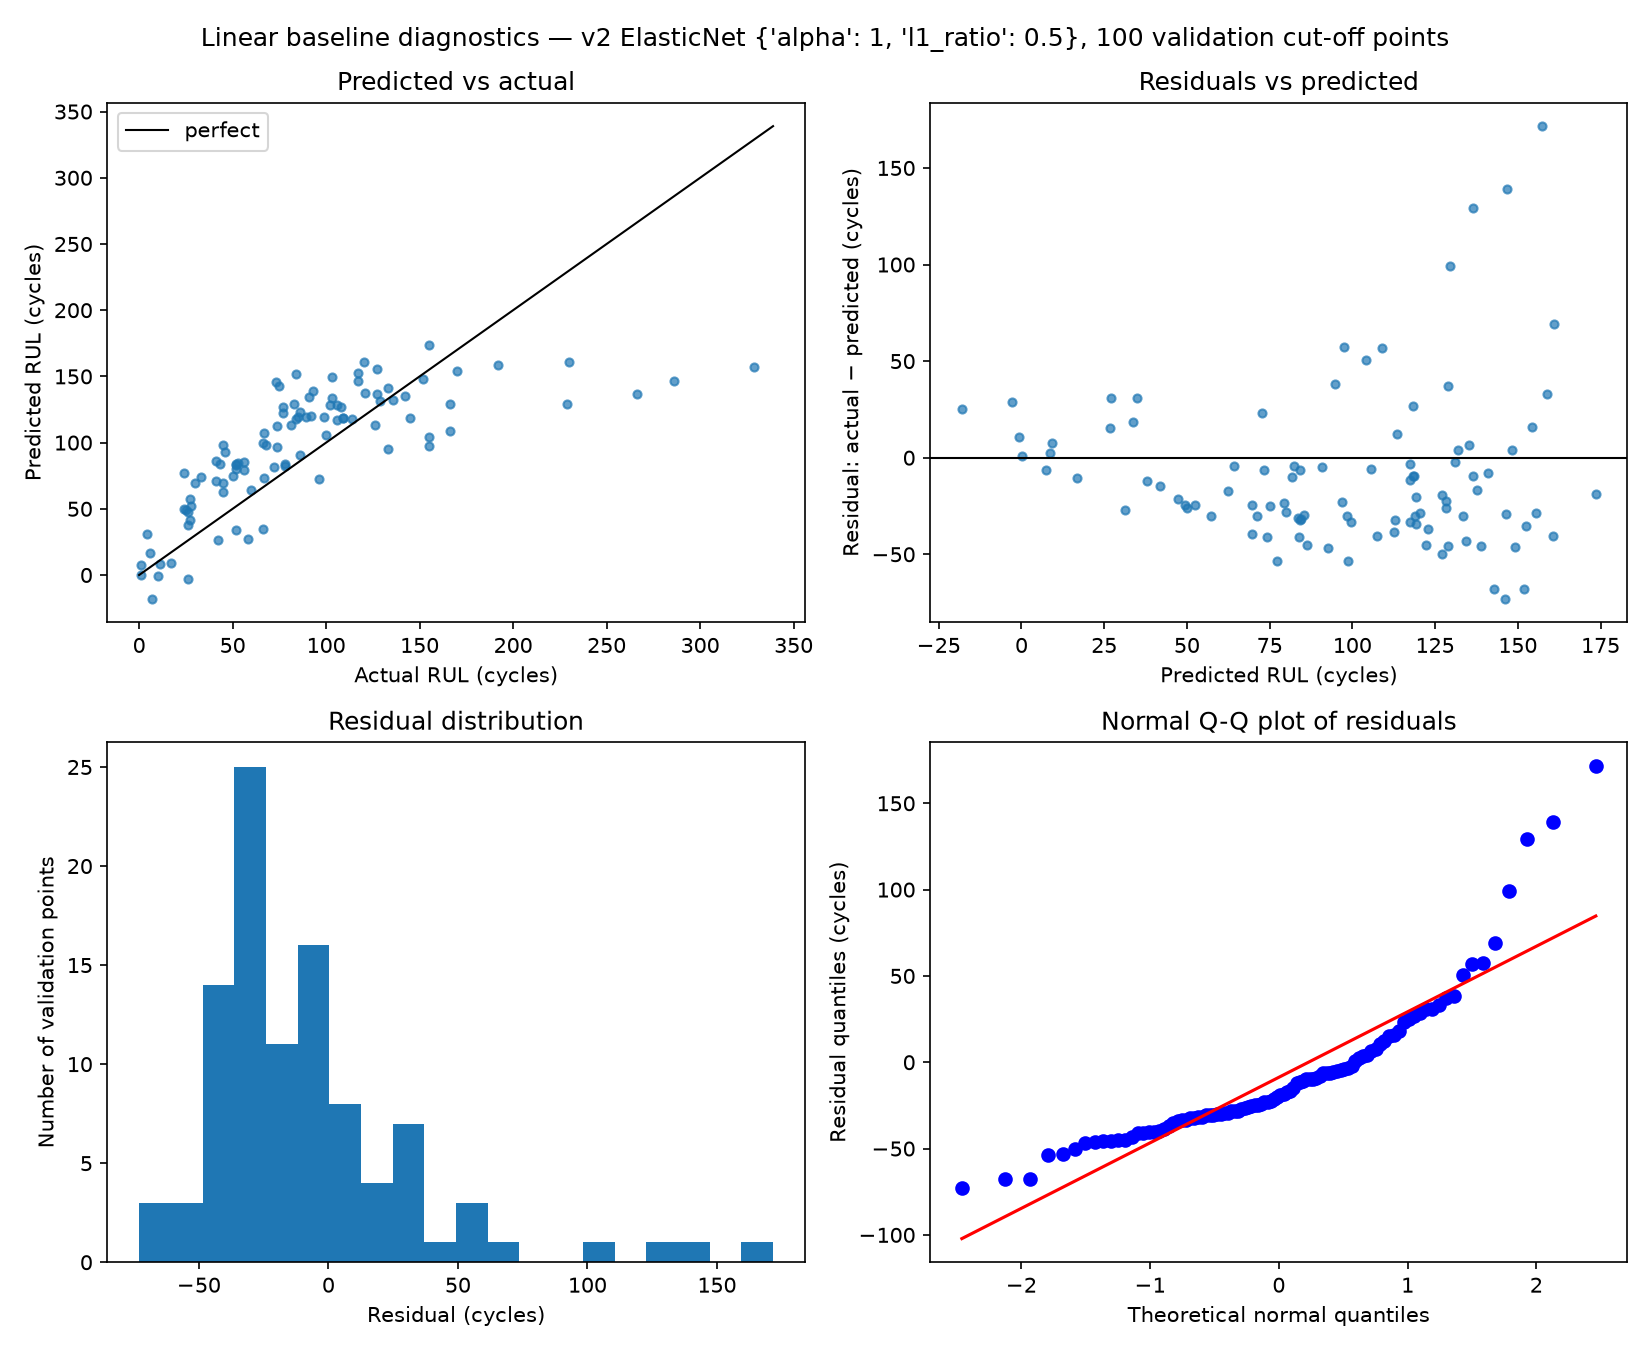
\includegraphics[width=\columnwidth]{../figures/linear_baseline_v2_validation_diagnostics.png}
  \caption{Diagnostics of the v2 linear baseline (Elastic Net) on the 100
  validation cut-off points: predicted vs.\ actual RUL, residuals vs.\
  prediction, residual histogram and normal Q-Q plot.}
  \label{fig:linear_diagnostics}
\end{figure}

\begin{figure}[t]
  \centering
  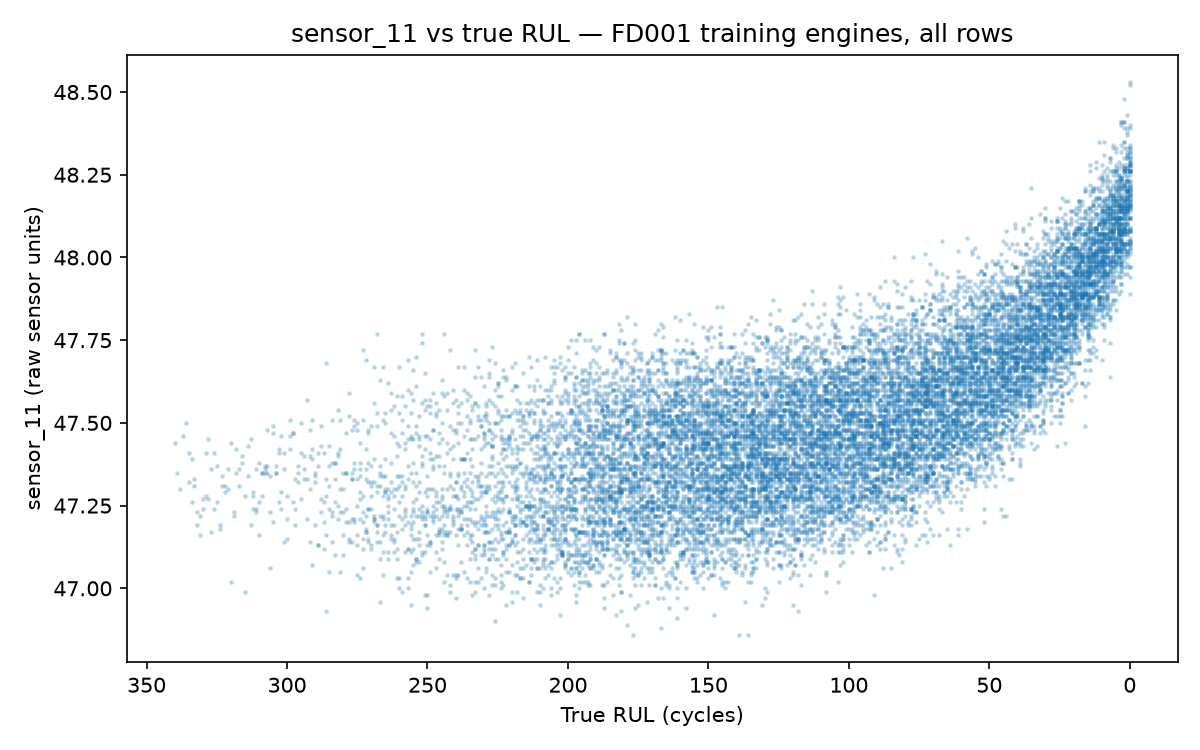
\includegraphics[width=\columnwidth]{../figures/linear_top_sensor_vs_rul.png}
  \caption{Raw \texttt{sensor\_11} against true RUL for all training rows. The
  reading changes little for large RUL and rises steeply near failure.}
  \label{fig:top_sensor}
\end{figure}
; assumes the main file sits in
% reports/latex/ so figures resolve via ../figures/.
% Needs: graphicx, booktabs. Table: run `python reports/latex/make_tables.py` first.

\section{Linear Baseline}
\label{sec:linear_baseline}

\subsection{Method}

As a reference point for all other models, we fit linear regression with two
feature sets:
\begin{itemize}
  \item \textbf{v1 (raw, 24 features):} the 3 operating settings and 21 raw
        sensor readings of the current cycle;
  \item \textbf{v2 (engineered, 57 features):} the cycle number, the 14
        informative sensors, and a trailing 10-cycle rolling mean, standard
        deviation and slope of each (Section~\ref{sec:evaluation} explains why
        features must be causal).
\end{itemize}
Each feature is standardised (zero mean, unit variance) using statistics from
the 80 training engines only. We compare ordinary least squares (OLS) with two
regularised variants:
\begin{itemize}
  \item \textbf{Ridge}, which adds an L2 penalty $\alpha \sum_j \beta_j^2$;
  \item \textbf{Elastic Net}, which mixes L1 and L2 penalties and can set
        coefficients exactly to zero.
\end{itemize}
The same small grids were used for both feature sets to avoid overfitting the
single validation split: $\alpha \in \{0.01, 0.1, 1, 10, 100, 1000\}$ for
Ridge, and $\alpha \in \{0.001, 0.01, 0.1, 1\}$ with L1 ratio
$\in \{0.2, 0.5, 0.8\}$ for Elastic Net. Within each feature set, the setting
with the lowest validation RMSE was chosen and then scored once on the test
set.

% Generated by reports/latex/make_tables.py from
% reports/results/linear_baseline_results.csv. Do not edit by hand.
\begin{table}[t]
\centering
\caption{Linear baseline on FD001 with raw (v1) and engineered (v2) features: best setting per model family. Validation: 100 cut-off points from 20 held-out engines. Test: 100 engines, scored once for the model chosen on validation within each feature set. Units: cycles.}
\label{tab:linear_baseline}
\resizebox{\columnwidth}{!}{%
\begin{tabular}{lllcccc}
\toprule
Features & Model & Hyperparameters & Val MAE & Val RMSE & Test MAE & Test RMSE \\
\midrule
v1 raw (24) & OLS & -- & 32.86 & 42.92 & 24.91 & 31.17 \\
v1 raw (24) & Ridge & $\alpha$=0.01 & 32.86 & 42.92 & -- & -- \\
v1 raw (24) & Elastic Net & $\alpha$=0.001, $\rho_{L1}$=0.8 & 32.87 & 42.92 & -- & -- \\
v2 engineered (57) & Elastic Net & $\alpha$=1, $\rho_{L1}$=0.5 & 31.66 & 41.77 & 23.61 & 29.04 \\
v2 engineered (57) & Ridge & $\alpha$=1000 & 31.93 & 41.89 & -- & -- \\
v2 engineered (57) & OLS & -- & 32.66 & 42.54 & -- & -- \\
\bottomrule
\end{tabular}}
\end{table}


\subsection{Results}

Table~\ref{tab:linear_baseline} lists the best setting of each model family.

\textbf{v2 is slightly better, and the gain comes from the cycle number.}
With v1 features, OLS, Ridge and Elastic Net all reach a validation RMSE of
42.92 cycles; OLS was kept as the simplest (test RMSE 31.17). With v2
features, Elastic Net ($\alpha = 1$, L1 ratio 0.5) reaches a validation RMSE
of 41.77 and a test RMSE of 29.04. The gain is consistent across validation,
all validation rows and test, but it is only 1--2 cycles. With about 20
independent validation engines, a gain of that size may partly be noise.

A validation-only ablation with the same model specification shows where the
gain comes from:
\begin{itemize}
  \item the cycle number plus the 14 raw sensors, with no rolling features,
        scores the same as the full v2 set (RMSE 41.74 vs.\ 41.77);
  \item removing the cycle number from v2 raises the RMSE to 43.33, slightly
        worse than v1.
\end{itemize}
For a linear model, the rolling mean, standard deviation and slope features
therefore add little once the cycle number is known. The cycle number acts as
a prior: engines that have already run longer have less life left on
average. The rolling features may still help non-linear models. The v2
Elastic Net remains the linear baseline, because it was chosen on validation
before the ablation was run.

\textbf{The linear model mostly underfits.} Training RMSE on all rows is high
for both feature sets (43.31 for v1, 39.30 for v2), so most of the error is
bias. The gap to validation widens slightly in v2 (to 47.25, against 49.72
for v1), which suggests a little more variance with 57 inputs. In v1,
regularisation therefore changes nothing. In v2 it improves on OLS by about
0.8 cycles (41.77 vs.\ 42.54). This is consistent with v2's correlated
inputs, but it is within the noise level, and the top v2 settings are
effectively tied. The best Ridge and Elastic Net strengths both lie at the
largest value tried. The grids were kept identical to v1 for comparability
and were not widened afterwards, because the test score had already been
seen.

\textbf{Uninformative and correlated inputs.} Seven raw features are constant
across the training engines (\texttt{setting\_3}, \texttt{sensor\_1},
\texttt{sensor\_5}, \texttt{sensor\_10}, \texttt{sensor\_16},
\texttt{sensor\_18} and \texttt{sensor\_19}). Seven raw feature pairs have an
absolute Pearson correlation of at least 0.8, the strongest being
\texttt{sensor\_9} and \texttt{sensor\_14} at 0.96. Individual coefficients
should therefore not be read as the effect of one sensor.

\textbf{Where the linear model fails.} For both feature sets, predictions
level off at about 150--175 cycles (Fig.~\ref{fig:linear_diagnostics}).
Engines with a true RUL between 200 and 330 cycles are predicted at roughly
130--160, and mid-range engines tend to be over-predicted.
Fig.~\ref{fig:top_sensor} suggests a likely reason. \texttt{sensor\_11}, the
raw input with the largest v1 coefficient, changes little while RUL is large;
it rises gradually from about RUL 150 and steeply near failure. A straight
line cannot represent this slow-then-accelerating pattern. This explanation
has not been tested directly. A few
predictions are negative (4 of 100 for v1, 3 of 100 for v2). They were left
unclipped, because clipping would change the model.

\textbf{Validation versus test.} Test errors are lower than validation errors
for both feature sets. A plausible but unconfirmed explanation is that the
validation cut-offs include very large RUL values that linear models miss. We
did not examine the test RUL distribution, since the protocol forbids it.

These results motivate two next steps:
\begin{itemize}
  \item non-linear models (trees) and sequence models, which can represent
        degradation that is flat and then accelerating;
  \item a capped RUL target, tested as a separate experiment.
\end{itemize}

\begin{figure}[t]
  \centering
  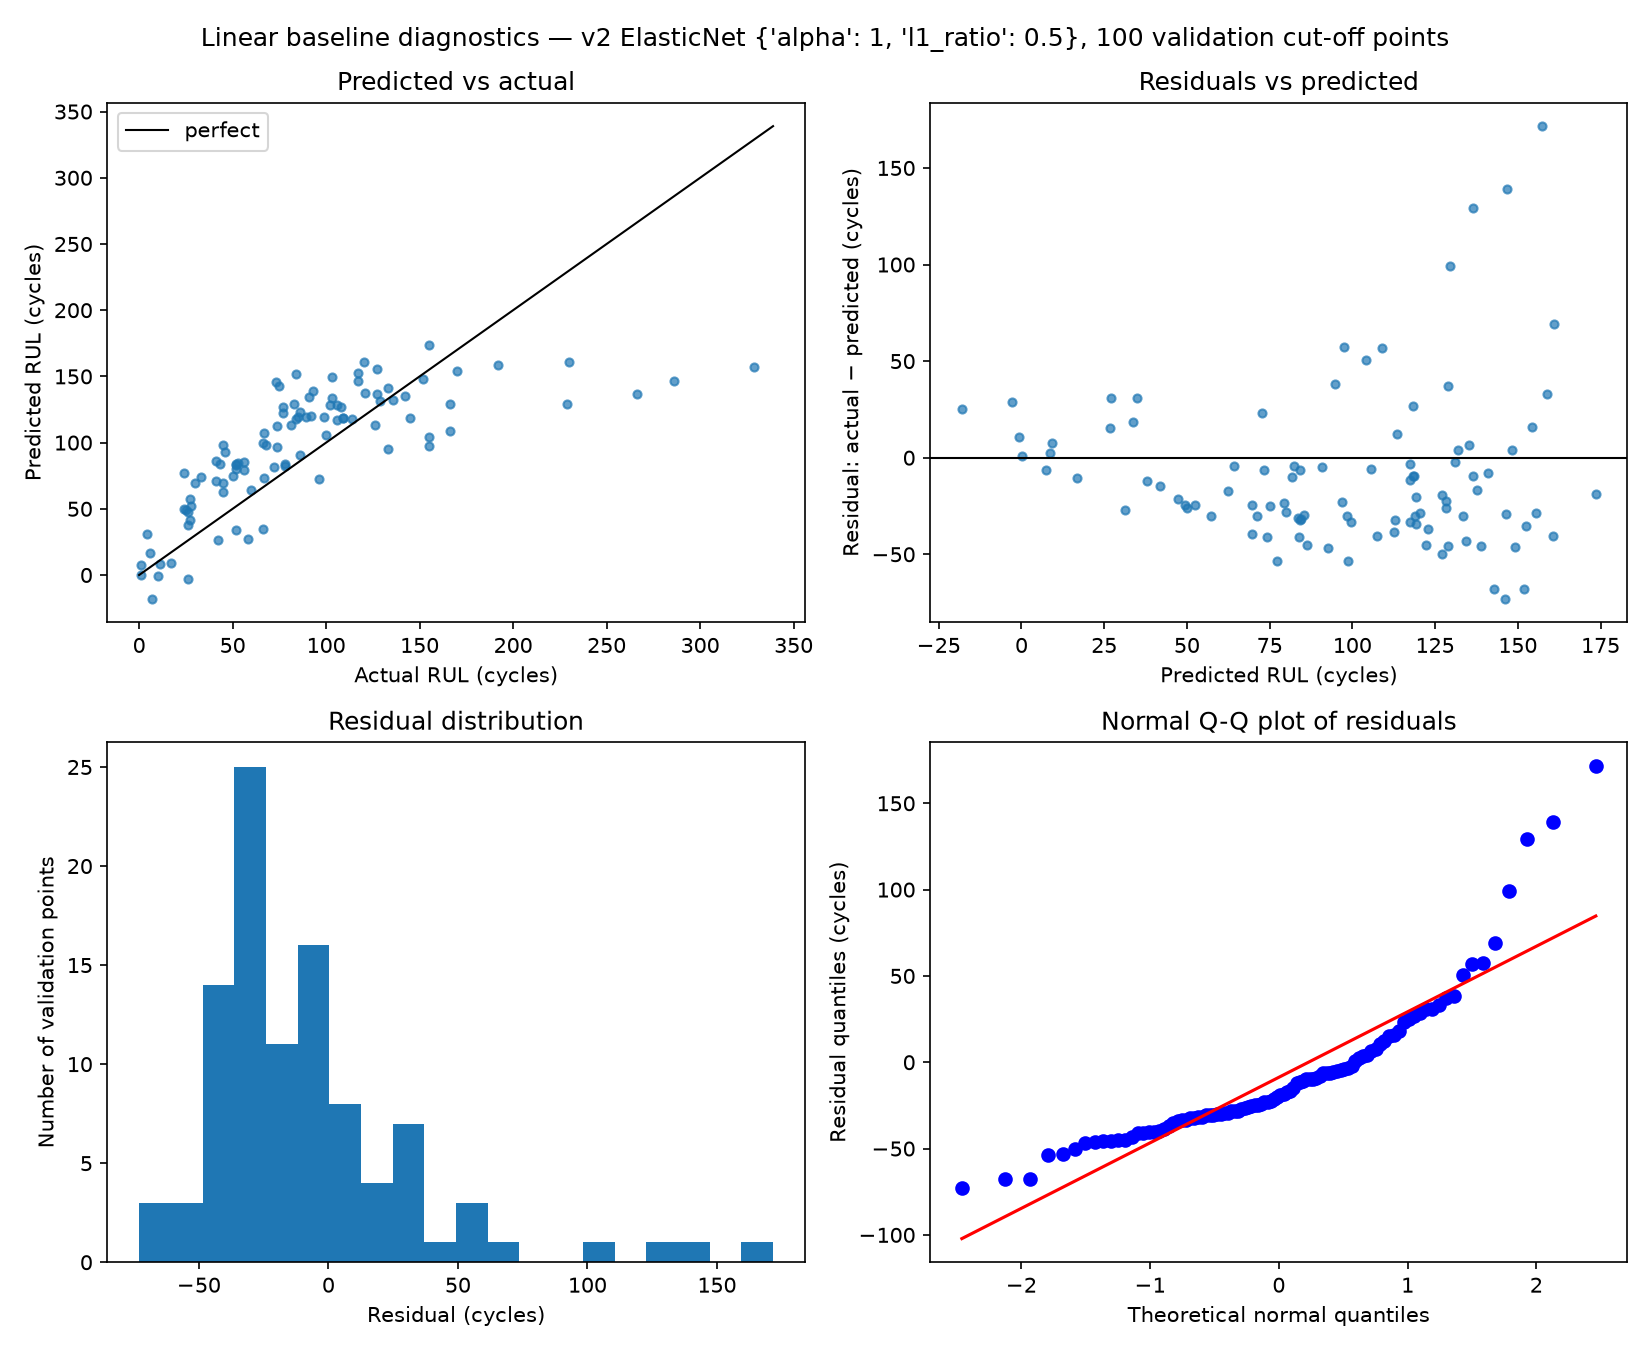
\includegraphics[width=\columnwidth]{../figures/linear_baseline_v2_validation_diagnostics.png}
  \caption{Diagnostics of the v2 linear baseline (Elastic Net) on the 100
  validation cut-off points: predicted vs.\ actual RUL, residuals vs.\
  prediction, residual histogram and normal Q-Q plot.}
  \label{fig:linear_diagnostics}
\end{figure}

\begin{figure}[t]
  \centering
  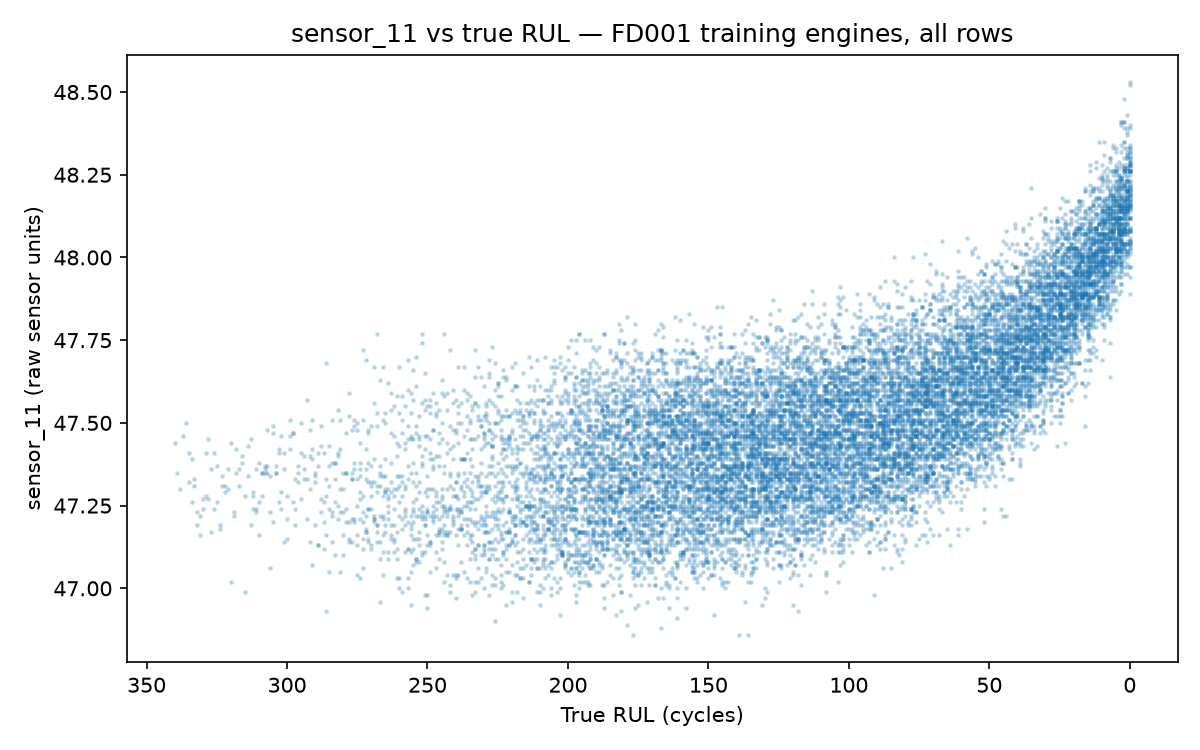
\includegraphics[width=\columnwidth]{../figures/linear_top_sensor_vs_rul.png}
  \caption{Raw \texttt{sensor\_11} against true RUL for all training rows. The
  reading changes little for large RUL and rises steeply near failure.}
  \label{fig:top_sensor}
\end{figure}
